\title{Epileptic Seizure Detection from EEG Signals with Autoencoded Features}
\author{Tuan Nguyen}
\date{\today}

\documentclass[12pt]{article}

\usepackage{url}
\usepackage{graphicx}
\usepackage{subcaption}
\usepackage{booktabs}

\newcommand{\myvec}[1]{\vec{#1}}

\begin{document}
\maketitle

\section{Definition}

\subsection{Project Overview}
\noindent
The domain of interest of this project belongs to physiological data such as electroencephalography (EEG), magnetoencephalography (MEG), electrocardiography (ECG) and the recorded signals from wearable devices. This project focuses on the EEG signals, which capture activities of brain neurons during a period of time. Different kinds of EEG data has been recorded from humans, for instance from those at rest, sleep~\cite{langkvist2012sleep}, during some periods of specific cognitive activities, or from patients with diseases such as Alzheimer's, Parkinson's, depression and epileptic seisures (\cite{andrzejak2001indications} and references thereof).

This project studies the classification problem on an EEG data set recorded from healthy volunteers and patients having epileptic seizures; solutions for this problem could be used to assist with detecting patients with the disease from their brain activity signals. Previous work on this data set focused mainly on extracting hand-crafted features to be used for classification. As examples, Nigam and Graupe \cite{nigam2004neural} extracted the spike amplitudes and frequency of the signals, feeding them into a neural network for classification; Guler et al.~\cite{guler2005recurrent} applied wavelet transformation to the signals to extract features, and classification was performed using a neuro-fuzzy system; Kannathal et al.~\cite{kannathal2005entropies} extracted entropy-based features for classification. This project, on the other hand, explores a type of autoencoders (e.g., ~\cite{bengio2007greedy}, \cite{vincent2010stacked}, \cite{boureau2008sparse}, \cite{kingma2013auto}) in order to learn features representing the EEG signals and then use them for classification.

\subsection{Problem Statement}
\noindent
This project aims to classify 1-second long EEG segments into one of the three classes: (1) healthy volunteers, (2) patients with epileptic seizures disease during seizure-free periods, and (3) patients with the disease during active seizure periods. It can be formally defined as follows.

\begin{itemize}
\item \textbf{Input:} training set $X = \langle \myvec{x}_1, \myvec{x}_2, ..., \myvec{x}_N\rangle$ of $N$ samples, where $\myvec{x}_i$ is a vector of $M$ electrical voltage values recorded in one second by an electrode at a specific point and time; target vector $y = \langle y_1, y_2, ..., y_N \rangle$ where $y_i \in \{1, 2, 3\}$ is the type of volunteers which the sample $\myvec{x}_i$ belong to. In the data set~\cite{andrzejak2001indications}, the targets $1, 2, 3$ respectively correspond to sets of volunteers $A + B$, $C + D$ and $E$.
\item \textbf{Output:} a hypothesis $f$ classifying a sample of $M$ electrical voltage values into one of the volunteer classes $\{1, 2, 3\}$.
\end{itemize}

The formation of the training set $X$ and target $y$ is discussed in Section~\ref{sec:data_set}. This project explores one of the following autoencoders for learning features of the training set $X$: ordinary autoencoders~\cite{bengio2007greedy}, denoising autoencoder~\cite{vincent2010stacked}, sparse autoencoder\cite{boureau2008sparse} and variational autoencoders \cite{kingma2013auto}. The extracted features are then tested with popular learning models (Decision Trees, K-Kearest Neighbors, Support Vector Machines and Feedforward Multi-layer Neural Networks) for classification (see Section~\ref{sec:solution}). Several metrics are used to evaluate the classifiers, discussed in Section~\ref{sec:metric}.

\subsection{Metrics}
\label{sec:metric}
The quality of the returned hypothesis is evaluated with an independent test set, created by $20\%$ of the given data set. The following measures are used to evaluate the performance of different classifiers:
\begin{itemize}
\item F1 score: this measure combines both the precision and recall as follows

\[
F_1 = 2 \times \frac{precision \times recall}{precision + recall}.
\]
\item Total accuracy: the total number of samples classified into the correct classes, which is still the most common measure used in practice.
\item Classification time: as suggested by Wulsin et al.~\cite{wulsin2011modeling}, this measure is important for applications monitoring EEG signals of patients in real time.
\end{itemize}

\section{Analysis}

\subsection{Data Exploration}

\label{sec:data_set}
The data set used in this study is provided with the work by Andrzejak et al.~\cite{andrzejak2001indications}, recording brain electrical activity of five sets of human volunteers:
\begin{itemize}
\item Set A: healthy volunteers in relaxed state with eyes open.
\item Set B: healthy volunteers in relaxed state with eyes closed.
\item Set D: epilepsy patients during seizure-free periods; the electrodes were implanted to record brain activity from within the epileptogenic zone.
\item Set C: epilepsy patients during seizure-free periods; the electrodes were implanted from the opposite hemisphere of the brain (compared to those in Set D).
\item Set E: same patients with sets C and D but activity were recorded from all electrodes during active seizures.
\end{itemize}

For each set of volunteers above, the data set contains 100 single-channel EEG segments of 23.6-sec duration. For this project each of these segments is divided into smaller segments of one second durations, which are considered stationary for EEG data~\cite{nigam2004neural}. These one second durations together define the training set $X$ in the problem statement, and the three sets of volunteers $A + B$, $C + D$ and $E$ define the target vector $y$ in the problem statement above.

\subsection{Exploratory Visualization}

\subsection{Algorithms and Techniques}
\label{sec:solution}

This project aims to use a type of autoencoders (~\cite{bengio2007greedy}, \cite{vincent2010stacked}, \cite{boureau2008sparse}, \cite{kingma2013auto}) that can learn to extract features of the training set $X$ for the purpose of classifying new sample of EEG segments. I propose to first try ordinary stacked autoencoders~\cite{bengio2007greedy}; the other autoencoders will be explored depending on the performance of the first one on this data set.

An ordinary autoencoder~\cite{bengio2007greedy} is a regular neural network which consists of the input layer, one hidden layer and the output layer such that the input and output layers have the same number of neurons. The first (lowest) autoencoder on the stack is trained to minimize the difference, defined for instance as the mean squared error, between the input batches of EEG segments and their output activations. The output activation of the hidden layer becomes the input to the second autoencoder on the stack, which is trained also to minimize the difference between its input and output layers. This process of adding more autoencoders continues in that fashion. Finally, the output layer of the entire stack is the output of the first autoencoder. The stacked autoencoders is therefore symmetrical with regard to the middle hidden layer: the first lower half acts as the encoder while the second higher half of the stack as the decoder. The output activations of the middle layer thus act as encoded features of the training set of EEG segments.

Depending on the performance of the above autoencoder in classifying the target classes of volunteers, I might also plan to train a stack of denoising autoencoders~\cite{vincent2010stacked} to extract features for the data set. At high level, this stack is much like the ordinary one except for the Gaussian noises added into the input layer, forcing the decoder to learn more meaningful features, potentially improve the performance in classification.

After the feature learning phase above, the output of the coding layer the network is considered the features representing the training set $X$. They are then used as input features of popular classification algorithms. This work considers the following classifiers: Decision Trees, K-Kearest Neighbors, Support Vector Machines and Feedforward Multi-layer Neural Networks. The hypothesis here is that the features learned automatically using autoencoders, together with one of these classifiers, provides comparable performance compared to the previous work (see Section~\ref{sec:benchmark}).

\subsection{Benchmark}
\noindent
Several previous work has been developed for the classification problem on the same data set~\cite{andrzejak2001indications}; the main contribution of most of these work, however, were on designing various hand-crafted features for the EEG signals. They might also be different from each other in the target classes of interest. As examples, Nigam and Graupe~\cite{nigam2004neural} used two features based on the spike information of the signals for further learning and detecting patients in set $E$ (thus, binary classification problem). Kabir et al.~\cite{kabir2016epileptic} extracted statistical features based on ``optimum allocation technique'' to be used with logistic model trees for classifying volunteers into the three classes that are of interest of this project. Guler et al.~\cite{guler2005recurrent} employed Lyapunov exponents based features for classification using recurrent neural networks where the target classes are three sets $A$, $D$ and $E$. On another data set, Wulsin et al.~\cite{wulsin2011modeling} learned features of second-long segments of EEG signals using Deep Belief Networks~\cite{hinton2006reducing} and classified them into ``clinically significant'' EEG classes. To the best of my knowledge, there was no previous work reporting the results of using autoencoders for the data set that this project is interested in.

The proposed method by Kabir et al.~\cite{kabir2016epileptic} on the data set of interest in this project outperforms many the state-of-the-art approaches using the same data set; among many other measures, the total accuracy of their approach was $95.3\%$. Since its target classes are the same with those of interest in this project, and their work represents a class of work using hand-crafted features, in my opinion it is reasonable to use the performance of their work as the baseline for the approach to be explored in this project. The hypothesis is that by using autoencoders, it is possible to learn a set of features automatically for classifying EEG signals with comparable results. The next section discusses measures to evaluate performance of classifiers in this domain.


\section{Methodology}

\subsection{Data Preprocessing}

The data set~\cite{andrzejak2001indications} contains 100 channels (or vector of voltage values) for each of the five sets of volunteers. Each channel is a vector of 4097 values that are EEG signals recorded in 23.6 seconds. The data set will be preprocessed as follows.
\begin{itemize}
\item Each channel is divided into 23 segments with equal length, each contains 178 values. These segments are marked with the target value $0$, $1$ or $2$ for the classes $A + B$, $C + D$ and $E$ of the original channel.
\item The resulting set of segments are splitted into training and test set (using StratifiedShuffleSplit function from Scikit-Learn).
\item The resulting set of segments in the training set are then normalized so that the values of EEG signals are in between $[0,1]$.
\end{itemize}

The data set was divided into three parts: training set ($60\%$), validation and testing sets ($20\%$ each). The testing set was set aside and not used in any ways during training or validating candidate models.

The training data was scaled into $[-1, 1]$ as follows (the formula):... This is to fit to ELU activation function.

The resulting scaling coefficients were then used to scale the testing and validation sets. This way we made sure that there were no information from the validation or testing sets used in any ways during training (data snooping).

\subsection{Implementation}

\subsection{Refinement}

\section{Results}

\noindent
\textbf{A. Randomly initialized vs. pretrained weights and biases:} We first examine the benefit of using weights and biases pretrained in unit autoencoders to initialize a multi-layer neural networks. Figure~\ref{fig:nopretrained_50_50} shows the learning curves for the training set (in red) and the validation set (in green) for a stack of two unit denoising autoencoders that were not pretrained. In other words, the weights and biases of the 2-layer fully connected network with $50$ neurons per layer, called $A_0$, were initialized randomly. Dropout technique with the rate $0.33$ (for input layer) and $0.5$ (for hidden layers) are used to cope with overfitting. During the training of this network, the best model was saved at step $3,878,215$ of batch updates, after which the network started to overfit to the training data (i.e., the validation curve began to go up). 

\begin{figure}
  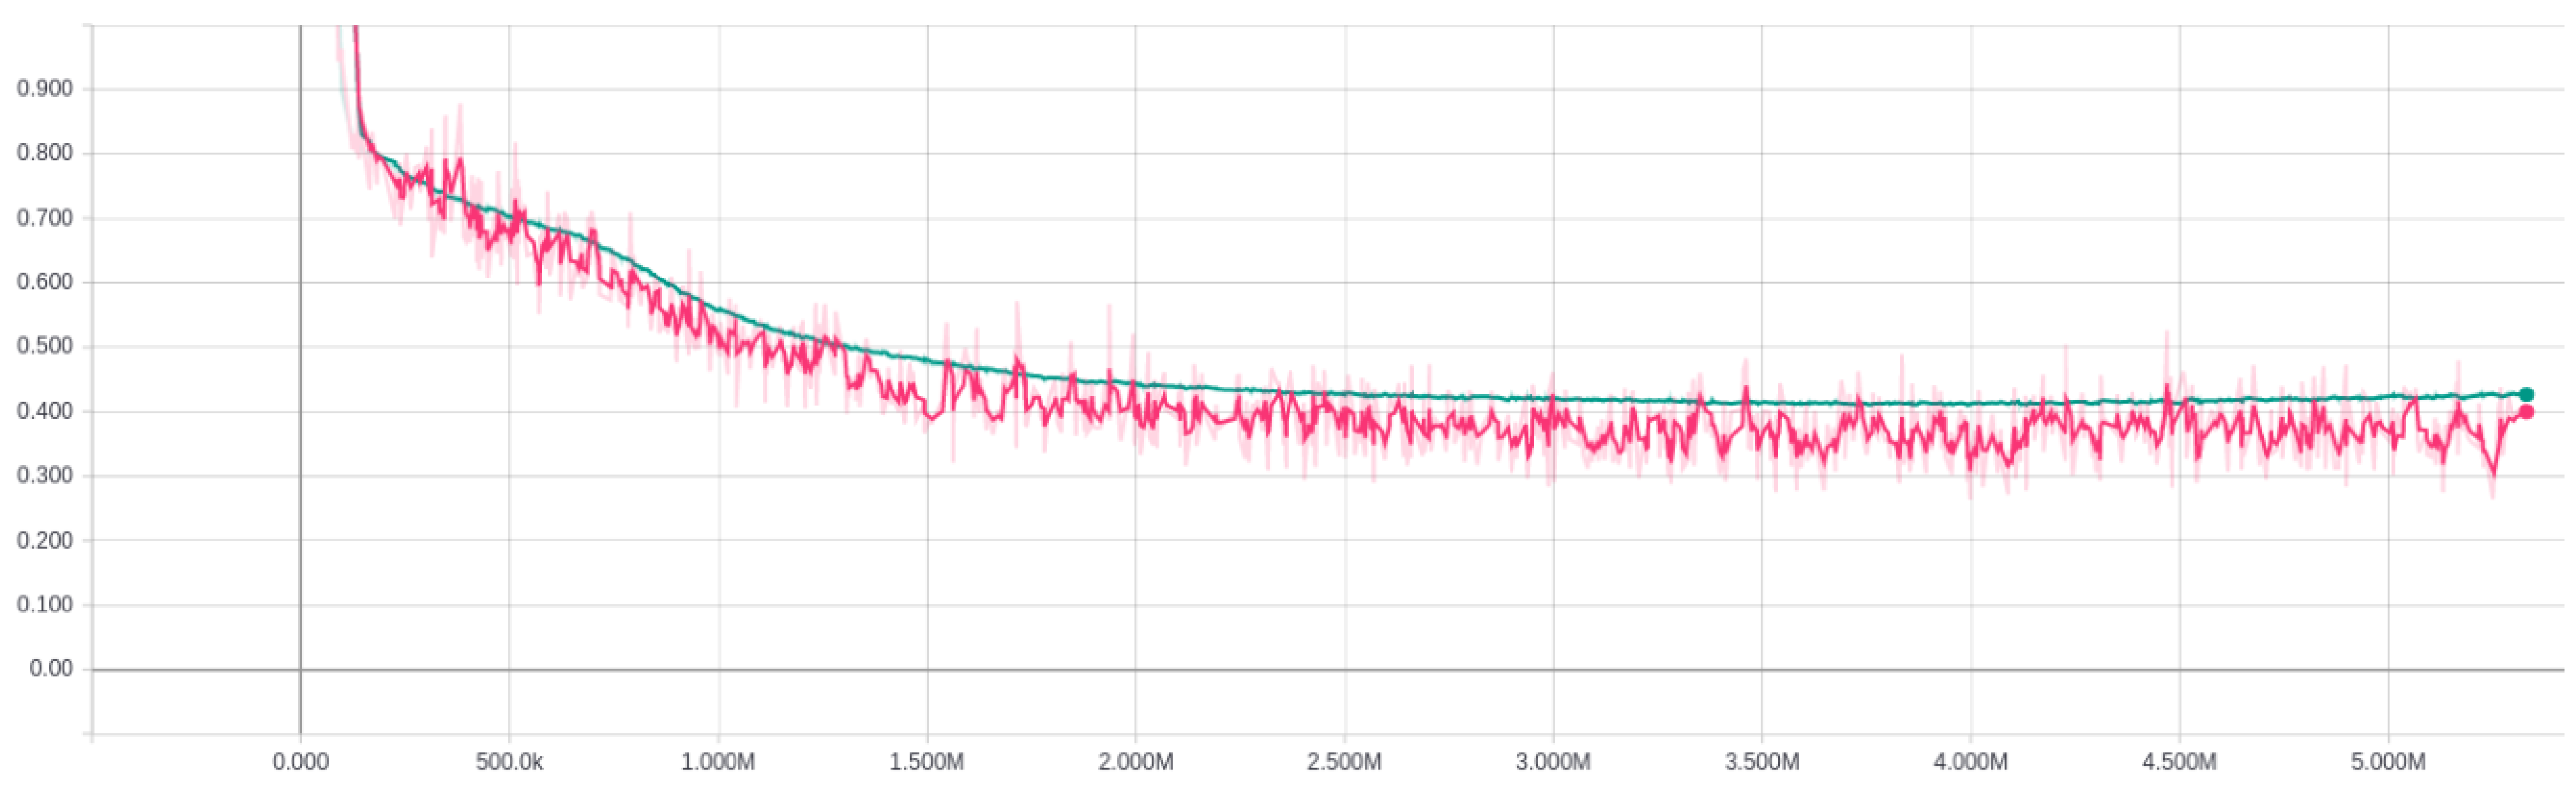
\includegraphics[width=\linewidth]{figures/nopretrained_50_50.eps}
  \caption{Cross-entropy error (Y-axis) on the training (red) and validation (green) sets of a 2-layer, 50 neurons each, fully connected network, called $A_0$, with randomly initialized weights and biases. Notice that the validation curve started to go up after about $3.8$ millions of batch updates, indicating the overfitting of the network.}
  \label{fig:nopretrained_50_50}
\end{figure}

Figure~\ref{fig:stack_50_50_dropout_elu} shows the learning curves for a similar stack as above but the two unit denoising autoencoders were pretrained to reconstruct their inputs, and the resulting weights and biases were used to initialize the stack before being fine-tuned. We could observe that the network did not overfit even after more than $18$ millions batch updates, which is much better than $A_0$. The cross-entropy error of this network on the validation set can also be seen as much better than from the one with randomly initialized weights and biases: less than $0.3$ vs. greater than $0.4$. This by definition results in a difference between $A_1$ and $A_0$ in terms of prediction accuracy on the validation, and importantly, the \emph{test} sets: $89.56\%$ vs. $87.52\%$, respectively. The accuracy errors by the two networks on the various sets are shown in Table~\ref{tab:Accuracy_A0_vs_A1}.

\begin{table}
\begin{center}
\begin{tabular}{|l||c|c|c|}
\hline
Network & Train set & Validation set & Test set \\ \hline \hline
$A_0$ & $89.59\%$ & $87\%$ & $87.52\%$ \\ \hline
$A_1$ & $92.75\%$ & $89.04\%$ & $89.56\%$ \\ \hline
\end{tabular}
\caption{Accuracy by networks $A_0$ and $A_1$ on training, validation and test sets.}
\label{tab:Accuracy_A0_vs_A1}
\end{center}
\end{table}

Although the network $A_1$ had a wider accuracy gap between its training and validation sets, it is important to stress that this gap did not appear to be widening, which was not the case for the network $A_0$. If the training were to be allowed on $A_1$, we would expect that its generalization capacity continues to be enhanced; the network $A_0$, however, overfitted early and would not have any benefits from further training.

\begin{figure}
  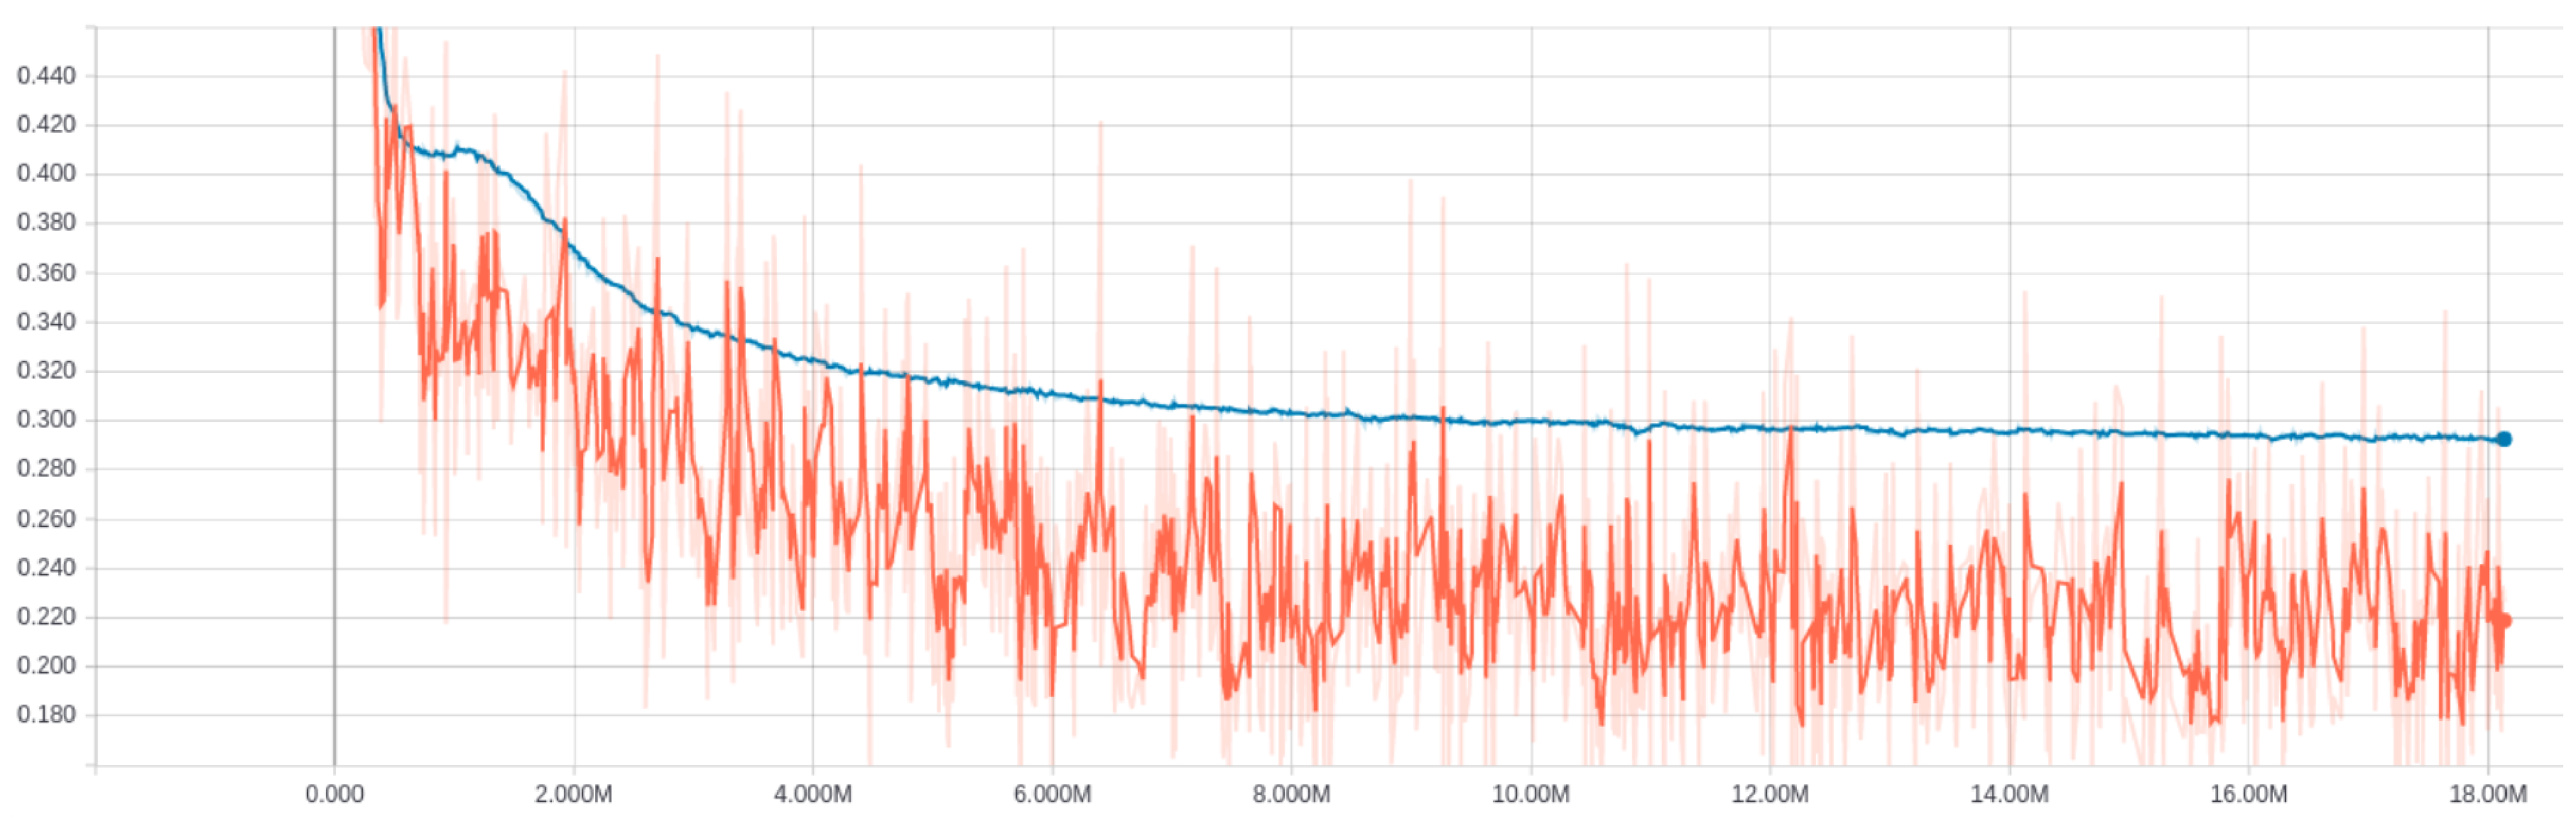
\includegraphics[width=\linewidth]{figures/stack_50_50_dropout_elu.eps}
  \caption{Cross-entropy error (Y-axis) on the training (red) and validation (green) sets of a 2-layer fully connected network, called $A_1$, whose weights and biases were initialized with pretrained values.}
  \label{fig:stack_50_50_dropout_elu}
\end{figure}

\vspace{5mm}
\noindent
\textbf{B. Ordinary vs. denoising autoencoders:}
\noindent
We now compare two types of autoencoders, ordinary and denoising, in terms of reconstructing orginal inputs and, more importantly, of learning representations for our classification problem. The denoising autoencoders here were those used to pretrain weights/biases of $A_1$, which learned their unique features by reconstructing the inputs from their corrupted version. The ordinary autoencoders had the same configuration with the other type (i.e., number of neurons, dropout rates for the hidden layer), except that they attempted to reconstruct the inputs from themself instead of their corrupted version. To test their representations in classifying the target signals, we constructed a 2-layer fully-connected neural network, called $B_0$, whose weights and biases were initialized from the two pretrained ordinary autoencoders.

Table~\ref{tab:reconstruction_errors} shows the reconstruction errors by two autoencoders of the above types used to construct the layers of networks $A_1$ and $B_0$. On both the training and validation sets, the ordinary autoencoders which processed the inputs directly resulted in more accurate reconstructed signals, i.e. with smaller errors, than those produced by the denoising counterpart; and this is true for autoencoders at two layers of the networks.

\begin{table}[!htbp]
\centering
\begin{tabular}{*5c}
\toprule
Autoencoder &  \multicolumn{2}{c}{Layer 1} & \multicolumn{2}{c}{Layer 2}\\
\midrule
{}         & Train   & Validation    & Train   & Validation\\
Ordinary   & 0.0015  & 0.0016   & 0.00051  & 0.00052\\
Denoise    &  0.0019  &  0.0021   & 0.0011  & 0.0011\\
\bottomrule
\end{tabular}
\caption{Reconstruction errors by ordinary and denoise autoencoders used at layer 1 and 2 of networks $B_0$ and $A_1$, respectively.}
\label{tab:reconstruction_errors}
\end{table}

The outperformance of ordinary autoencoders in reconstructing the input signals, however, did not transform to its classification performance. Figure~\ref{fig:stack_50_50_dropout_elu_clean_input} shows the cross-entropy errors by the network $B_0$: it was expressive enough and achieved $97.13\%$ accuracy on the training set, however overfitted early after step $1,675,620$ of batch updates. The accuracy of the resulting best model on the validation and testing sets were $90.47\%$ and $91.78\%$, respectively. (The corresponding statistics by $A_1$ was presented in the previous result section.) Both the about $7\%$ performance gaps on between the training and the two independent sets, and the $>1\%$ gap between the validation and test sets indicate that this model suffers from high variance. The network $A_1$, which used features extracted through reconstructing corrupted inputs, as shown in Figure~\ref{fig:stack_50_50_dropout_elu}, provided a comparable and more reliable accuracy performance on unseen data.

\begin{figure}
  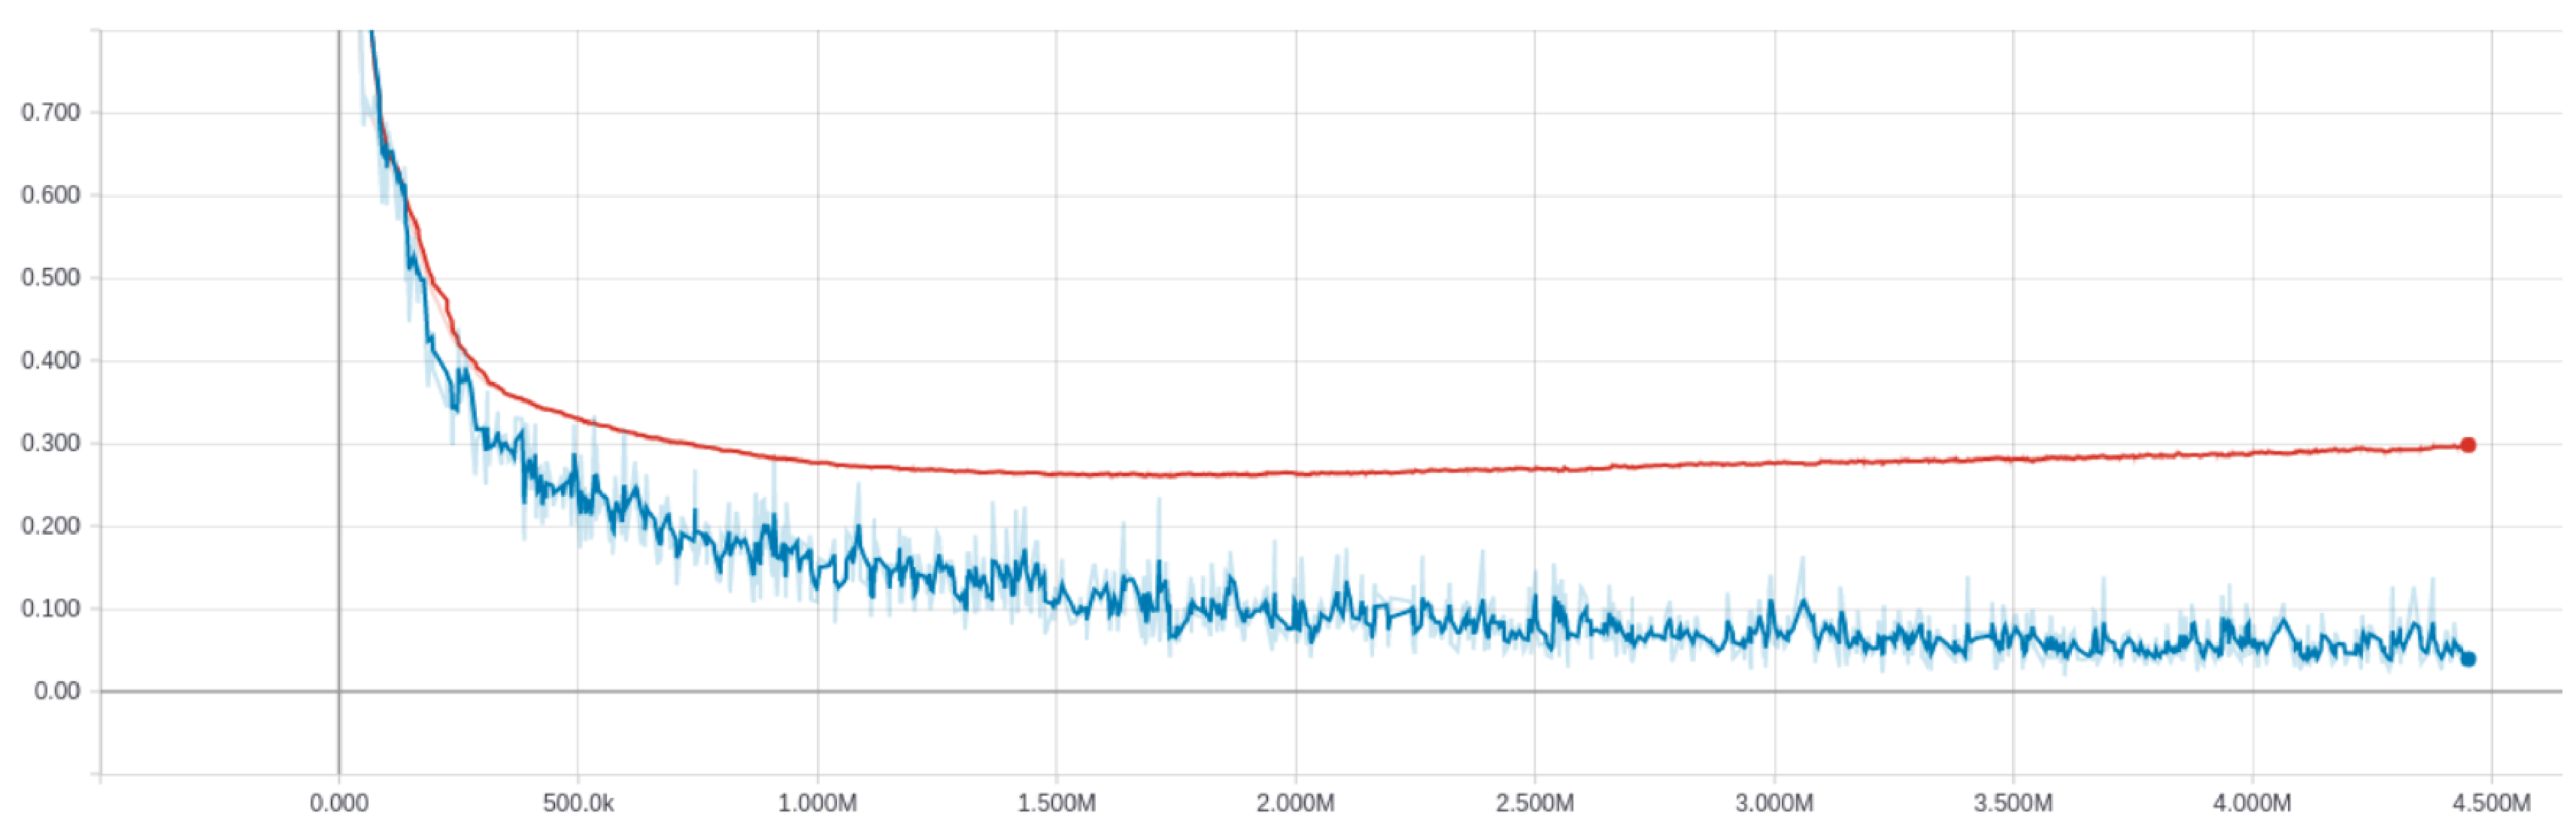
\includegraphics[width=\linewidth]{figures/stack_50_50_dropout_elu_clean_input/stack_50_50_dropout_elu_clean_input.eps}
  \caption{Cross-entropy error (Y-axis) on the training (green) and validation (red) sets of a 2-layer fully connected network, called $B_0$, with inputs not being corrupted during training.}
  \label{fig:stack_50_50_dropout_elu_clean_input}
\end{figure}

Perhaps one explanation for the above difference could be that since the two networks were the same except for the clean vs. the corrupted inputs that they processed, the noises introduced into the inputs helped the network $A_1$ learned features more essential to the original inputs; when used for classification task, these features resulted in much less overfitting model compared to those simply learned from an identity function of the clean inputs. Although it is hard for humans to make sense the features learned by the two networks to represent brain activity signals (in contrast to interpretable features in image domains), it is interesting to see what the neurons were ``excited'' about after the learning process. Figure~\ref{fig:weights_stack_50_50_dropout_elu_clean_input} shows the weights of six randomly chosen neurons learned by the first ordinary autoencoder used in network $B_0$: we could observe that the weights did not appear to learn any interesting patterns after reconstructing the original inputs.

\begin{figure}
\begin{subfigure}{.5\textwidth}
  \centering
  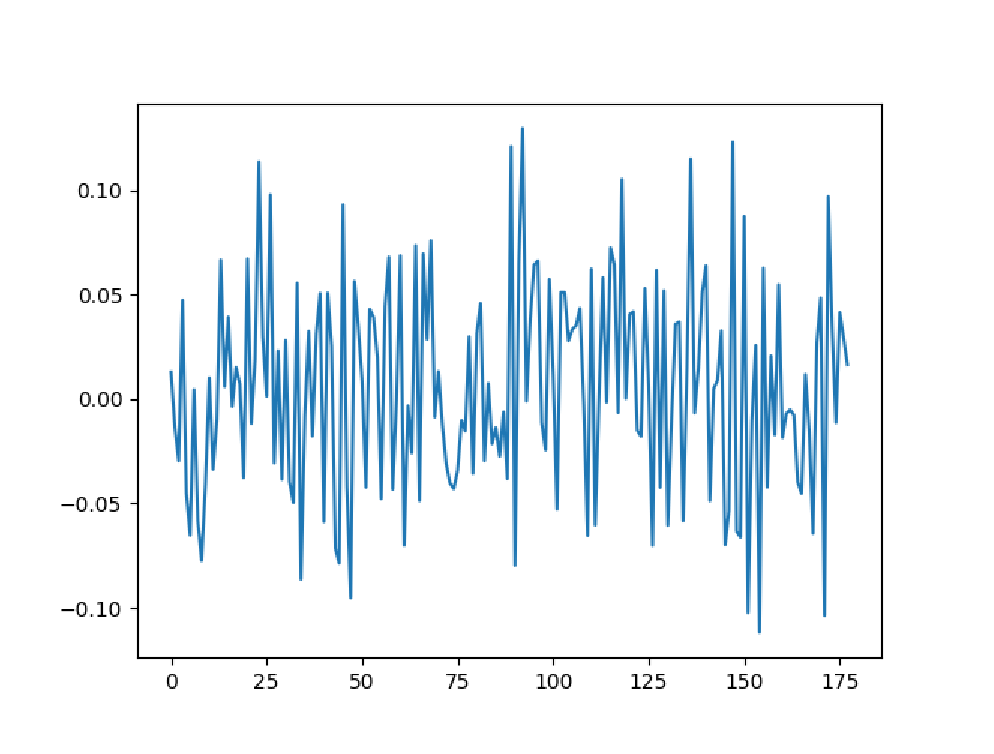
\includegraphics[width=.8\linewidth]{figures/stack_50_50_dropout_elu_clean_input/weights_neuron_0.eps}
\end{subfigure}%
\begin{subfigure}{.5\textwidth}
  \centering
  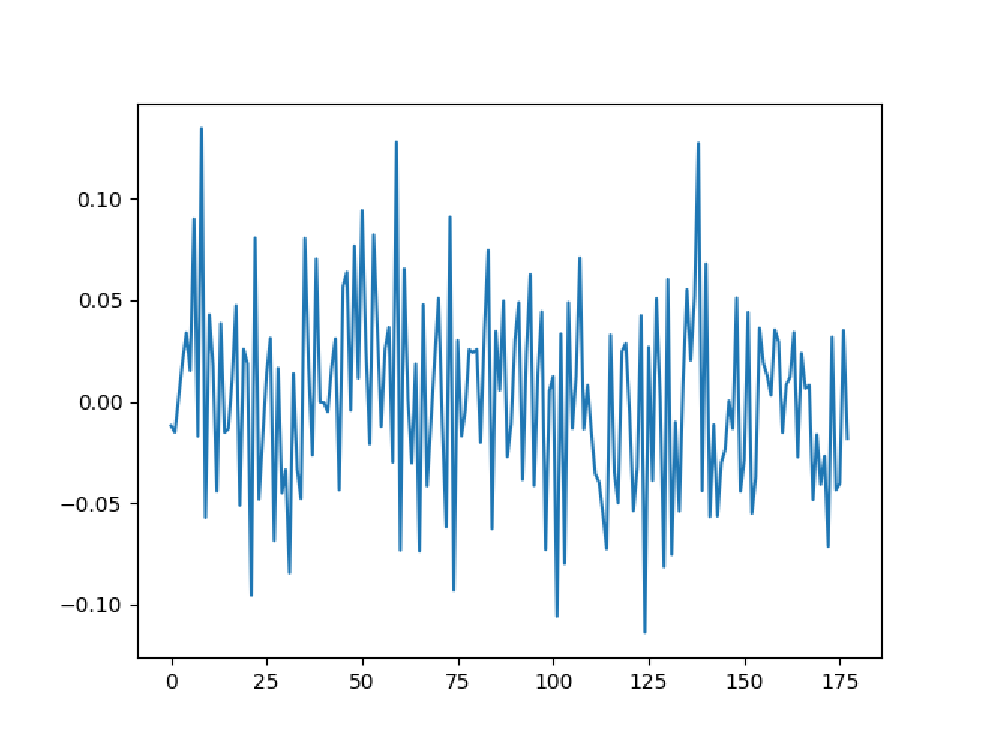
\includegraphics[width=.8\linewidth]{figures/stack_50_50_dropout_elu_clean_input/weights_neuron_1.eps}
\end{subfigure}

\begin{subfigure}{.5\textwidth}
  \centering
  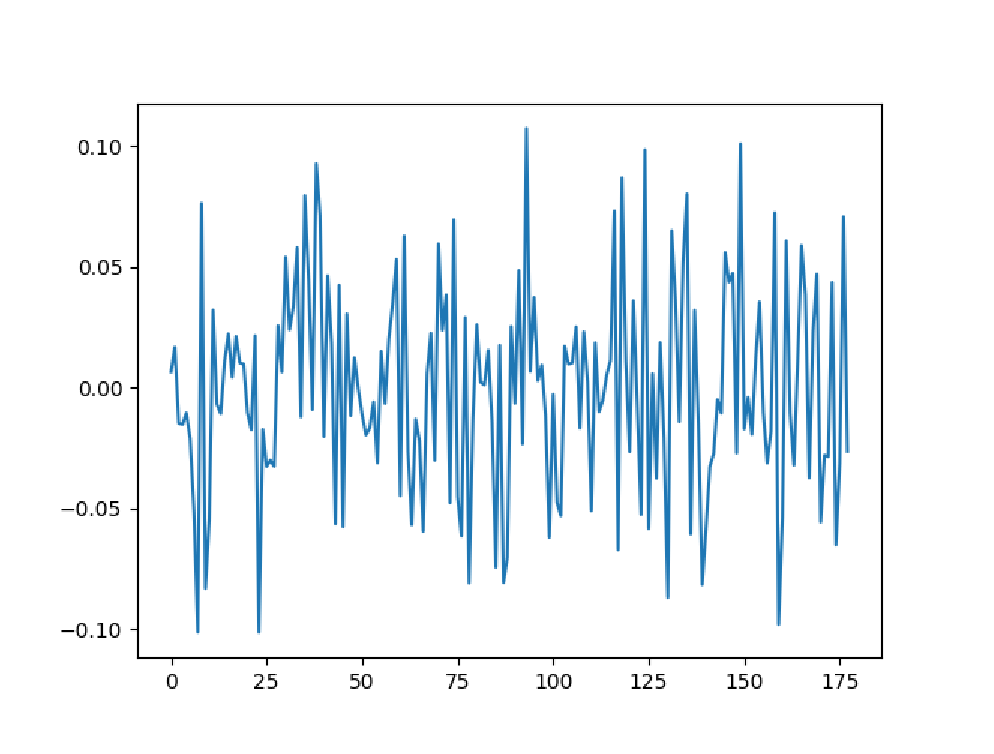
\includegraphics[width=.8\linewidth]{figures/stack_50_50_dropout_elu_clean_input/weights_neuron_2.eps}
\end{subfigure}%
\begin{subfigure}{.5\textwidth}
  \centering
  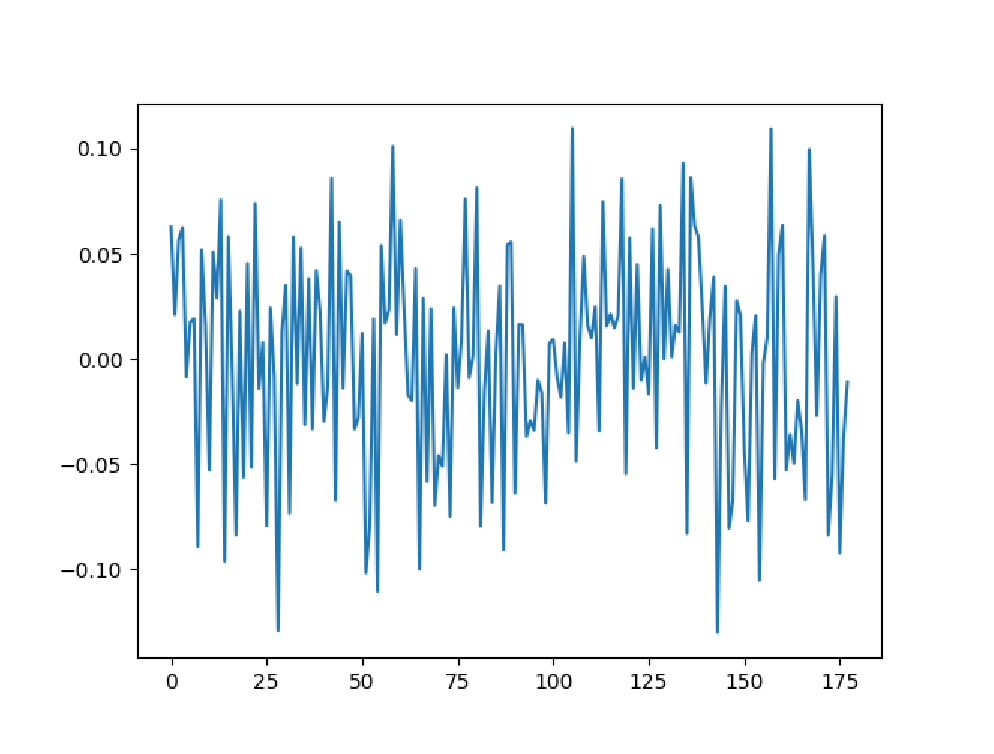
\includegraphics[width=.8\linewidth]{figures/stack_50_50_dropout_elu_clean_input/weights_neuron_3.eps}
\end{subfigure}

\begin{subfigure}{.5\textwidth}
  \centering
  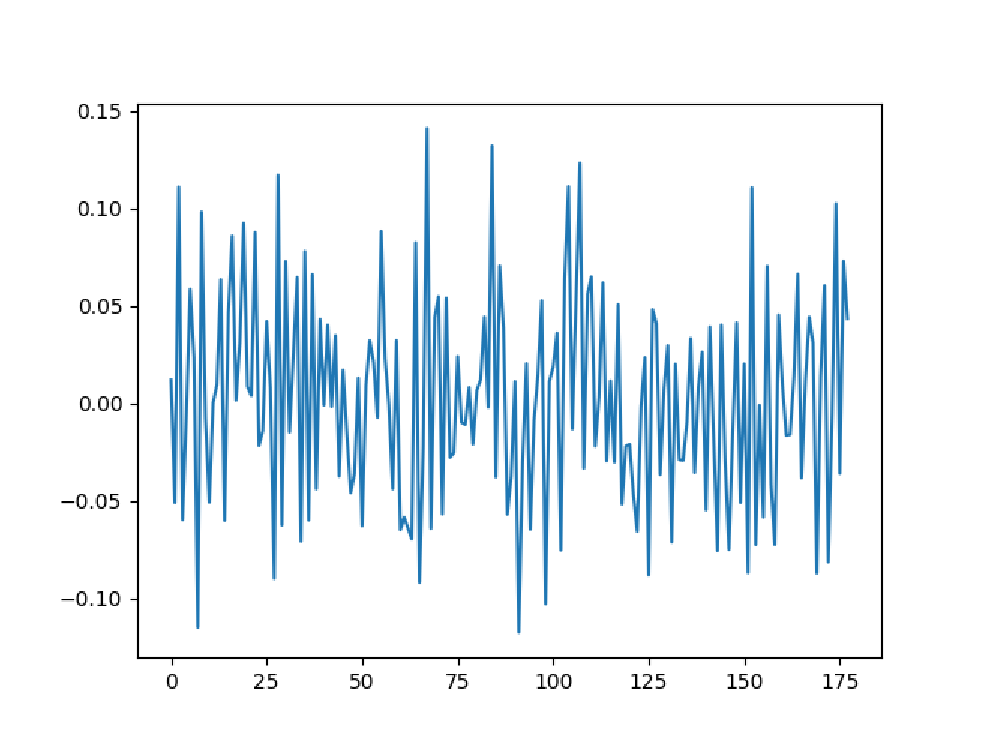
\includegraphics[width=.8\linewidth]{figures/stack_50_50_dropout_elu_clean_input/weights_neuron_4.eps}
\end{subfigure}
\begin{subfigure}{.5\textwidth}
  \centering
  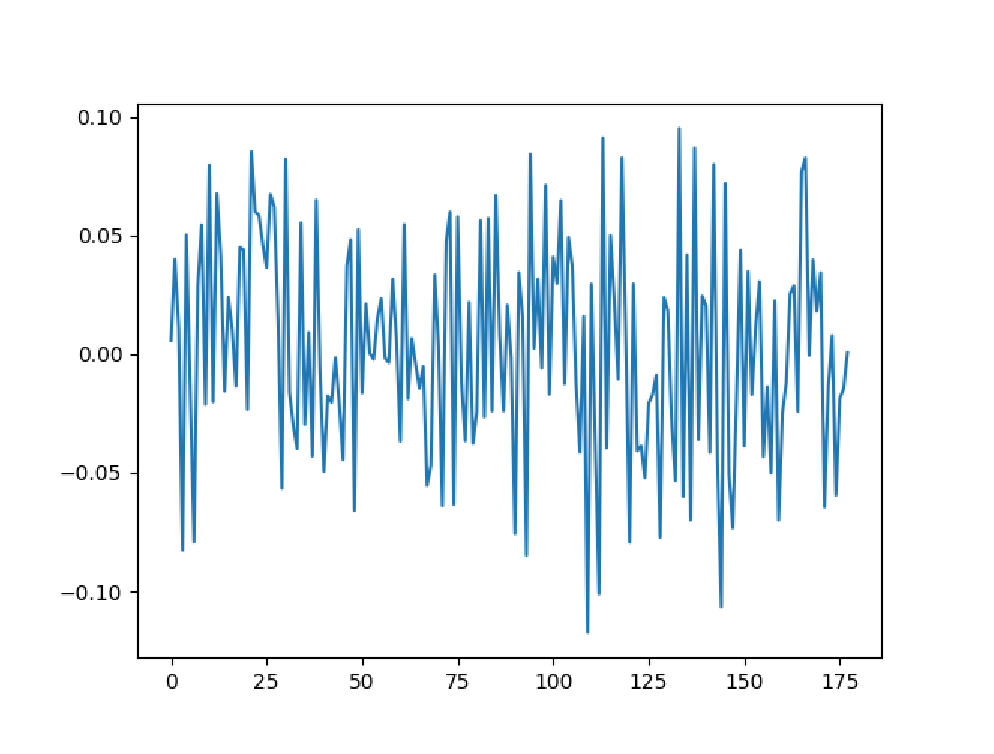
\includegraphics[width=.8\linewidth]{figures/stack_50_50_dropout_elu_clean_input/weights_neuron_8.eps}
\end{subfigure}
\caption{Weights of six neurons, chosen randomly, learned by the first ordinary autoencoder used in network $B_0$ after reconstructing the original (uncorrupted) inputs.}
\label{fig:weights_stack_50_50_dropout_elu_clean_input}
\end{figure}

For the same set of neurons, Figure~\ref{fig:weights_stack_50_50_dropout_elu} shows their weights learned by the denoising autoencoder used in the first hidden layer of network $A_1$ after reconstructing the inputs from their corrupted version. As opposed to those in Figure~\ref{fig:weights_stack_50_50_dropout_elu_clean_input}, these weights appear to reflect some specific patterns that the neurons were adapted to. Similar contrasts could also be observed for autoencoders at the second layers of the networks $B_0$ and $A_1$.

\begin{figure}
\begin{subfigure}{.5\textwidth}
  \centering
  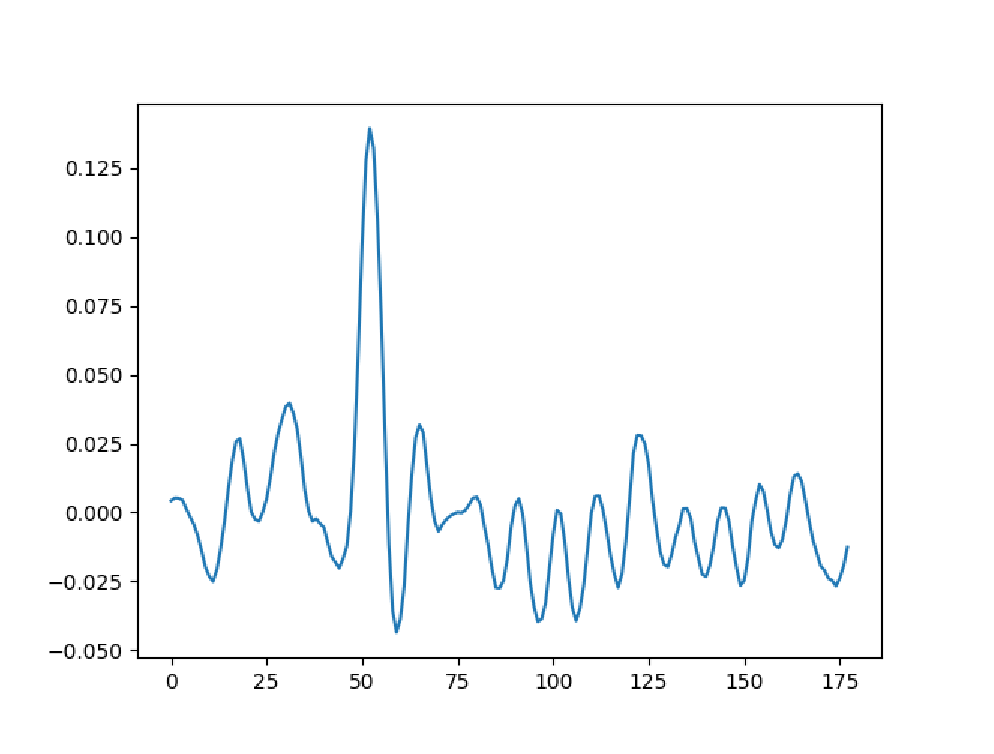
\includegraphics[width=.8\linewidth]{figures/stack_50_50_dropout_elu/weights_neuron_0.eps}
\end{subfigure}%
\begin{subfigure}{.5\textwidth}
  \centering
  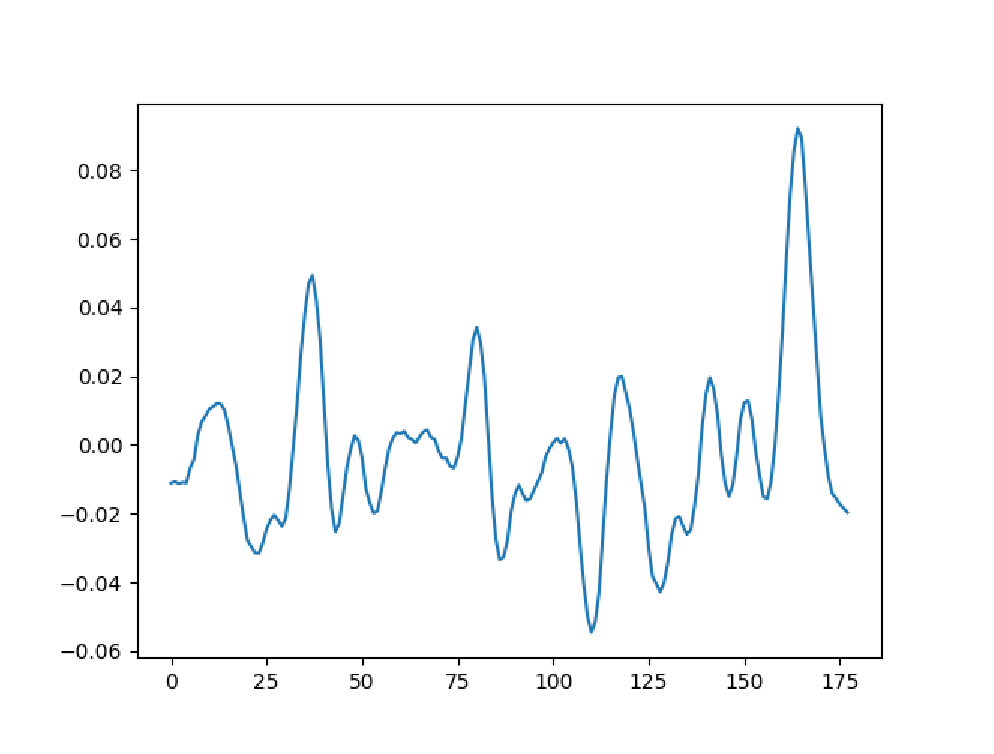
\includegraphics[width=.8\linewidth]{figures/stack_50_50_dropout_elu/weights_neuron_1.eps}
\end{subfigure}

\begin{subfigure}{.5\textwidth}
  \centering
  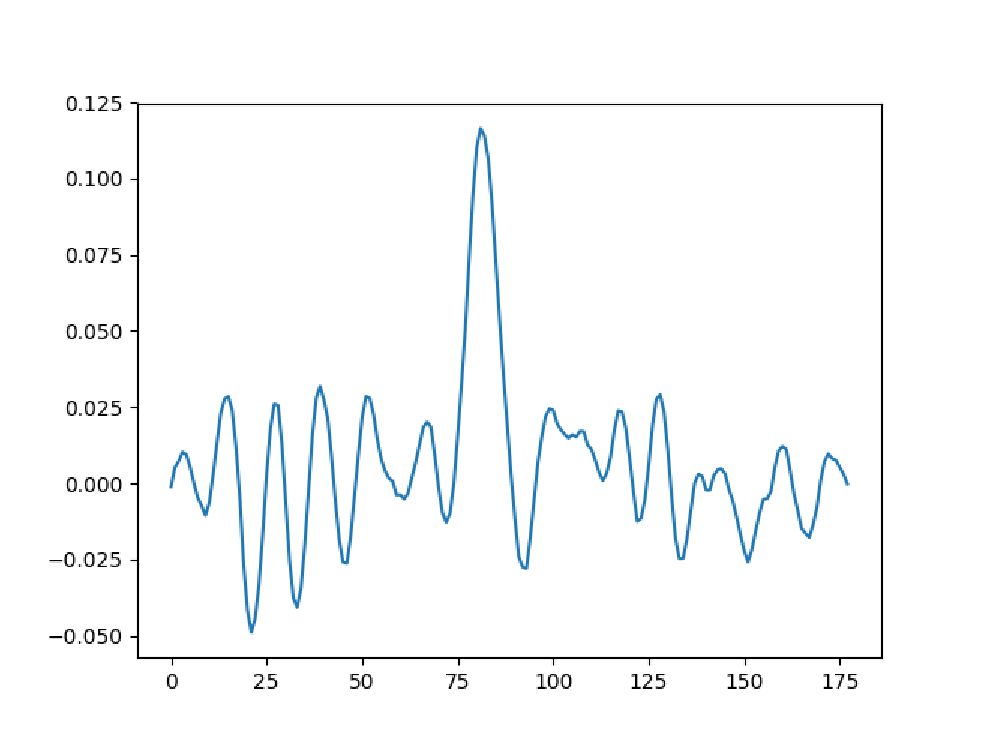
\includegraphics[width=.8\linewidth]{figures/stack_50_50_dropout_elu/weights_neuron_2.eps}
\end{subfigure}%
\begin{subfigure}{.5\textwidth}
  \centering
  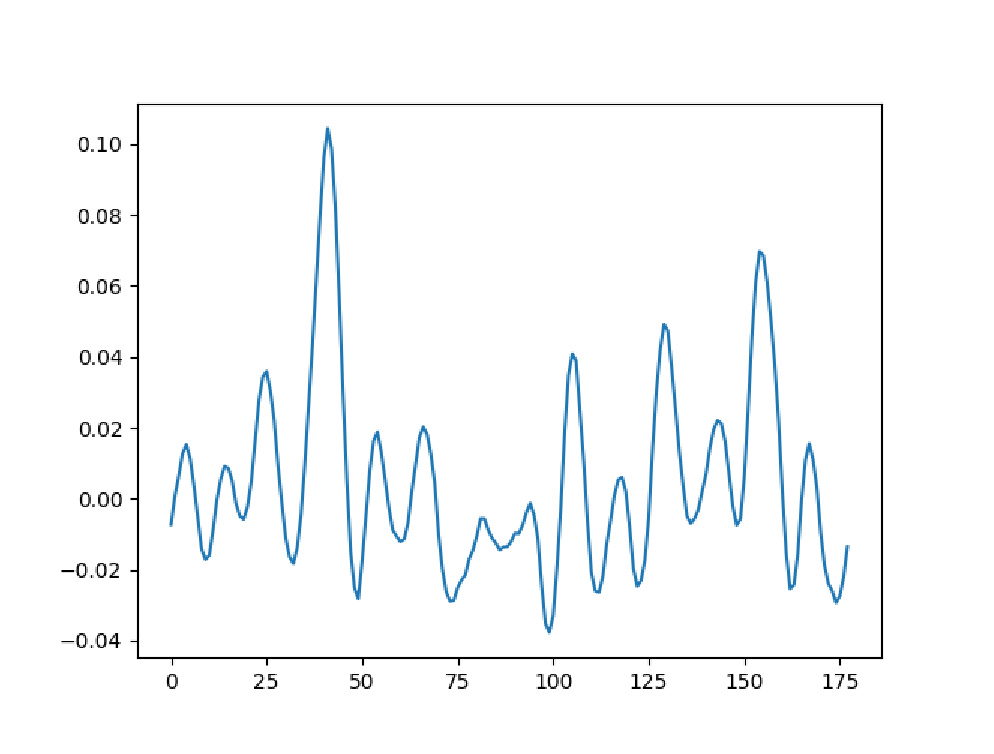
\includegraphics[width=.8\linewidth]{figures/stack_50_50_dropout_elu/weights_neuron_3.eps}
\end{subfigure}

\begin{subfigure}{.5\textwidth}
  \centering
  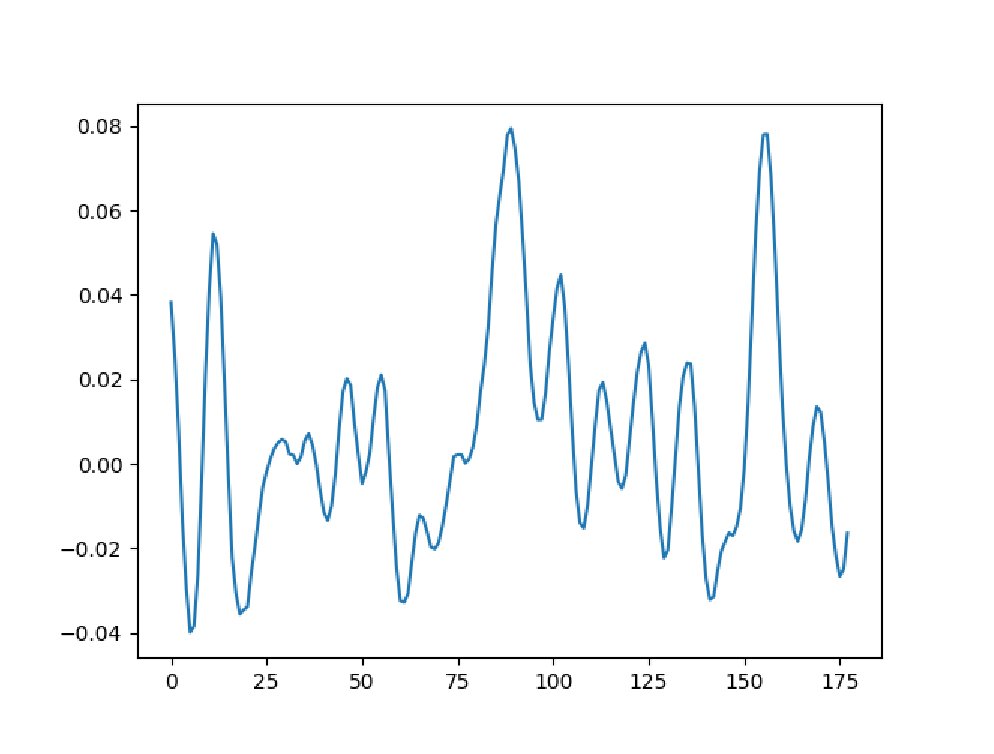
\includegraphics[width=.8\linewidth]{figures/stack_50_50_dropout_elu/weights_neuron_4.eps}
\end{subfigure}
\begin{subfigure}{.5\textwidth}
  \centering
  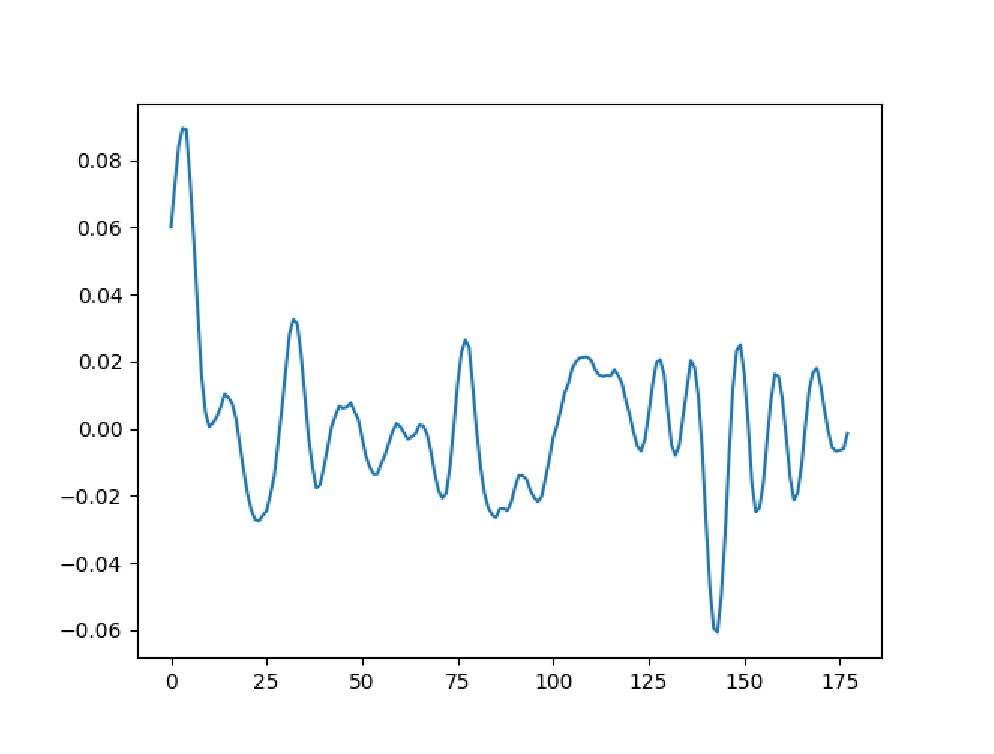
\includegraphics[width=.8\linewidth]{figures/stack_50_50_dropout_elu/weights_neuron_8.eps}
\end{subfigure}
\caption{Weights of the corresponding six neurons in Figure~\ref{fig:weights_stack_50_50_dropout_elu_clean_input} learned by the first ordinary autoencoder used in network $A_1$ after reconstructing the corrupted inputs.}
\label{fig:weights_stack_50_50_dropout_elu}
\end{figure}

\textit{Comparision on networks of 75-neuron layers}: Table~\ref{tab:Accuracy_B1_vs_B2} shows the accuracy performances of networks $B_1$ and $B_2$ with 2 layers fully connected networks, each having 75 neurons. They differed in exactly the same way $B_0$ and $A_1$ were distinguished: $B_1$ reconstructed the original signals from clean inputs, whereas $B_2$ did that from the corrupted inputs.

\begin{table}
\begin{center}
\begin{tabular}{|l||c|c|c|l|}
\hline
Network & Train set & Validation set & Test set\\ \hline \hline
$B_1$ & $97.3\%$ & $89.61\%$ & $90.22\%$\\ \hline
$B_2$ & $94.28\%$ & $89.99\%$ & $90.69\%$\\ \hline
\end{tabular}
\caption{Accuracy by networks with 2 layers of 75 neurons $B_1$ and $B_2$ on training, validation and test sets. $B_1$ reconstructed the original signals from themselves, and $B_2$ did so from the corrupted inputs.}
\label{tab:Accuracy_B1_vs_B2}
\end{center}
\end{table}


\vspace{5mm}
\noindent
\textbf{C. Gaussian noisy inputs vs. dropout inputs:}

\vspace{5mm}
\noindent
\textbf{D. Denoising autoencoders with dropout: number of neurons and layers}


\section{Conclusion}
\noindent

\bibliographystyle{abbrv}
\bibliography{report}

\end{document}
